\documentclass[12pt]{article}
\usepackage[T1]{fontenc}
\usepackage{graphicx}
\usepackage{listings}
\usepackage{xcolor}
\lstset { %
    language=C++,
    backgroundcolor=\color{black!5}, % set backgroundcolor
    basicstyle=\footnotesize,% basic font setting
}


\begin{document}


\title{Traveling Salesman Problem with Parallel Genetic Algorithm}
\author{Niklas Karlsson \\ Student ID: 0151055513}
\date{}
\maketitle

\newpage


\section{Introduction}

When trying to solve computationally highly-demanding problems, it is important to make the most
of the available resources. in the traveling salesman problem, the goal is to compute the shortest
route possible from a list of cities and their coordinates. For a circular route, where starting
point does not matter, with $N$ cities there are $(N-1)!$ possible solutions causing the problem to
scale badly as number of cities grows. To solve this, many different algorithms have been
developed, including genetic algorithms.

Genetic algorithms mimic the principles of evolution in the search for better solutions by
allowing the different solutions to generate children and improving each generation. This method
speeds up the process of finding good solutions, as not every possible solution is needed to be
explored.

Parallelization of algorithms is an important tool in high performance computing. By allowing
the computations to be divided to multiple processors, the time used can be halved by
doubling the amount of processes in the ideal case. Not all algorithms can be parallelized, so it
is important to construct the algorithm in such a way that computations can be easily divided to
processes, and so that the communication between the processes is as efficient as possible.

In this report we will take a look at an implementation of parallel genetic algorithm for a
travelling salesman problem. We will look at how to implement different aspects of genetic
algorithms to a \lstinline!C++! code and how the computation time scales as number of processeses
is increased.


\section{Traveling Salesman Problem}

Traveling salesman problem (TSP) is an old optimization problem, dating back to atleast 1800th
century \cite{Bryant}. The problem description is that you are given a list of cities and their
their coordinates. From this list of cities, you are to construct a route such that each city is
visited exectly once and the route will end at the starting point. The challenge is to find the
optimal route that minimizes the total distance traversed.

What makes this problem intriguing from algorithmical standpoint, is that the problem is
NP-hard, meaning that there are no guaranteed ways of finding the optimal solution in polynomial
time. This constraint is often evaded by the use of different algorithms, which will find a near
optimum solution while reducing the time required drastically. We will focus on how genetic
algotihms (GA) and especially the one implimented for this report, are used to find solutions for
the traveling salesman problem.


\section{Genetic Algorithm}

Genetic algorithms are based on the idea of evolution as seen in nature. Different solutions are
searched by first guessing a population of solutions, which are then allowed to mate,
generating new and ideally better results. Genetic algorithms can be divided into five steps
\cite{Bryant}.
\begin{itemize}
\item Encoding
\item Evaluation
\item Crossover
\item Mutation
\item Decoding
\end{itemize}

Next let us go through description of each step and how they have been employed in the code I
have written.

\subsection{Encoding}

Encoding is the first step of approaching the problem, as it defines the way how the problem is
written in the code. In genetic algorithms, a solution is called a chromosome, which would
correspond to the solution written for example as a string or a list. Each element in the
chromosome is called a gene, corresponding possibly to an integer or a character in the chromosome.
There are multiple ways of encoding a chromosome, but in the case of TSP, it makes sense to
encode the chromosomes as a vectors of cities (genes) in the order as they are traversed.

In the code, I have constructed a class for holding information and defining operations to be
done on the chromosome \lstinline?class Chromosome?. Here inside of the class, encoding is
\begin{lstlisting}
  vector<int> genes(chromosome_length);
\end{lstlisting}

In the vector, each city is identified with an integer.


\subsection{Evaluation}

In genetic algorithms, each chromosome is given a fitness score determining how good of a solution
the chromosome is. In the case of TSP, where the optimum solution is one where the least amount of
distance is covered, it is logical to use the total distance of the route as the fitness score for
the chromosome, where a lower fitness corresponds to a better solution. In this implementation, I
have chosen to precalculate all the distances into a distance matrix, where distances can be easily
found from by the indices of the cities

\begin{lstlisting}
for (int i = 0; i < chromosome_length - 1; i++) {
  for (int j = i + 1; j < chromosome_length; j++) {
    float dist = d(cities[i], cities[j]);
    dist_matrix[i][j] = dist_matrix[j][i] = dist;
  }
}
\end{lstlisting}

The distance between cities $i$ and $j$ is calculated in the matrix as
\begin{lstlisting}
float d(City i, City j)
{
  return sqrt( pow(j.x - i.x, 2) + pow(j.y - i.y, 2) );
}
\end{lstlisting}

where \lstinline!i.x! and \lstinline!i.y! are the x- and y-coordinates of the cities. The
precalculation of the distances helps with computatuion time, as the distances do not need to be
calculated on the go as needed.

\subsection{Crossover}

Crossover refers to the process of generating children from parent chromosomes. This is where the
evolution idea of the algorithm is implemented. Crossover is a process where population (collection
of chromosomes) passes a generation. Some genetic algorithms are based on the idea of survival of
the fittest, where only the fittest chromosomes are allowed to generate cildren. The process of
generating a child from parents can be totally random or heuristics can be used.

In this implementation, all chromosomes are randomly chosen a pair, from which two children are
created. In the case of odd number of chromosomes in a population, one chromosome is left without
a pair remaining unaltered in the next generation. The children replace replace their parents
each generation, meaning that the size of the population remains constant.

The heurestic algorithm implimented here goes as follows:

\begin{enumerate}
\item Choose as the first city of the child, the first city of either of the parents.
\item Next, choose as the second city, the second city of the parent which minimizes the
  distance between the two cities.
\item If the city already exists in child, choose the second city from the other parent.
\item If that city already exists in the child too, randomly choose a city not in the child yet.
\item Repeat steps 2 to 4 until all cities exist in the child.
\end{enumerate}

This method tries to improve each generation by combining the best parts of both parents in the
children generated. The two children are generated from two parents so that the starting cities of
the children come from both parents. The algorithm is implemented within the \lstinline!Chromosome!
class as follows

\newpage

\begin{lstlisting}
Chromosome generate_child(Chromosome *chrom)
{
  Chromosome child;
  set<int> pool = geneset;
  child.genes[0] = genes[0];
  pool.erase(genes[0]);
  for (int i=1; i<chromosome_length; i++) {
    
    if (child.check_if_city_exists(genes[i],i)) {
      if (child.check_if_city_exists(chrom->genes[i],i)) {
        int r_member = getRandomSetElement(pool);
        child.genes[i] = r_member;
        pool.erase(r_member);
        continue;
      } else {
	  child.genes[i] = chrom->genes[i];
	  pool.erase(child.genes[i]);
	  continue;
      }
	
    } else if (child.check_if_city_exists(chrom->genes[i],i)) {
      child.genes[i] = genes[i];
      pool.erase(child.genes[i]);
      continue;
	
    } else {
      float dist1 =
        dist_matrix[child.genes[i-1]-1][genes[i]-1];
      float dist2 =
        dist_matrix[child.genes[i-1]-1][chrom->genes[i]-1];
      if (dist1 <= dist2) {
        child.genes[i] = genes[i];
        pool.erase(child.genes[i]);
      } else {
        child.genes[i] = chrom->genes[i];
        pool.erase(child.genes[i]);
      }
      
    }
      
  }
  return child;
}
\end{lstlisting}

\subsection{Mutation}

It is often the case that in genetic algorithms, the solutions can converge around a local minimum
(or maximum, depending on the problem), preventing the algorithm to sufficiently search the whole
solution space and possibly missing more optimal solution further from the local minimum. The
mutation process allows some chromosomes to escape the local mimimum, to possibly find better
solutions elsewhere in the solution space.

Mutation is typically a completely random process, where after crossover a random chromosome is
chosen and it is modified in some randomized way. In this implementation, the chosen chromosome is
altered in such way, that two cities are are randomly chosen and then their places are swapped.
The genes of a chromosome are mutated as follows
\begin{lstlisting}
  void mutate()
  {
    unsigned int r_num1 = chrom_dist(gen);
    unsigned int r_num2 = chrom_dist(gen);
    int tmp = genes[r_num1];
    genes[r_num1] = genes[r_num2];
    genes[r_num2] = tmp;
  }
\end{lstlisting}

\subsection{Decoding}

Decoding is the final step of the solution where the result of the algorithm is turned back into a
concrete solution. In TSP problem not much decoding is needed since the solution already is the
list of cities in the order of which they are traversed. In using genetic algorithms, it might be
difficult to know when to stop the computations and extract the solution. Sometimes different
stopping criterias are used, which could be ones like if the best solution has not changed in $n$
many steps, then the computations are stopped.

In this case, the number of generations is set at
the beginging of computations so that the wall clock times between different runs can be compared.
After the computations are finished, the code will save the best chromosome found during the run
into a file.

\section{Parallelization}

To decrease the computation time of the algorithm, it is beneficial to try to parallelize the
algorithm. There are several ways one could try to parallelize the algorithm used here. The method
choosen for this implementation is to divide the population of chromosomes to different processes
using MPI. Each process will take care of the crossover and mutation of its own population. To
ensure the spreading of genes between the processes, every process will send a determined amount of
its best chromosomes to neighbouring process every $n$th generation. This process is called
migration. The interval of migration is given as
an argument in the beginging of the run. The chromosomes cycle through the processes in the fashion
as shown in the figure, where each process sends its best chromosomes to the process with id
larger by one, and from last to first.
\begin{figure}[h]
  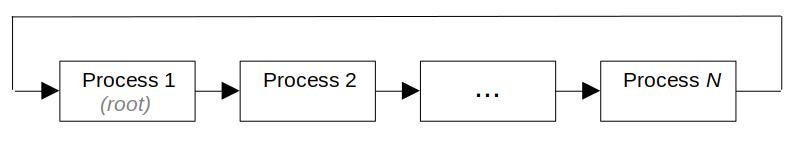
\includegraphics[scale=0.475]{migration.png}
\end{figure}

The process is handled by MPI in the following manner (population is sorted by fitness before):
\begin{lstlisting}
  for (int j = 0; j < mig_count; j++) {
    vector<int> send_buff = population[j].genes;
    vector<int> recv_buff(chromosome_length);
    MPI_Sendrecv(send_buff.data(), chromosome_length, MPI_INT,
                 dest, 0, recv_buff.data(), chromosome_length,
                 MPI_INT, source, 0, MPI_COMM_WORLD,
                 MPI_STATUS_IGNORE);
    population[j].genes = recv_buff;
  }
\end{lstlisting}

The root process will after migration also collect the best results from each process to rember
which chromosome so far has been the best solution:
\newpage
\begin{lstlisting}
   vector<int> recv_bests_buff(id_count * chromosome_length);
   vector<int> displ(id_count);
   vector<int> counts(id_count);
   for (int i=0; i < id_count; i++) {
     displ[i] = i * chromosome_length;
     counts[i] = chromosome_length;
   }
   MPI_Gatherv(population[0].genes.data(), chromosome_length,
               MPI_INT, recv_bests_buff.data(), counts.data(),
               displ.data(), MPI_INT, root, MPI_COMM_WORLD);
      
   if (id == root) {
     for (int j = 0; j < id_count; j++) {
       best_chromosomes[j].genes =
       vector<int>(recv_bests_buff.begin()+j*chromosome_length,
                   recv_bests_buff.begin() +
                   (j+1)*chromosome_length);
     }
     calculate_population_fitness(best_chromosomes);
     sort_population(best_chromosomes);
     if (best_chromosomes[0] < best_so_far) {
       best_so_far = best_chromosomes[0];
     }
   }
 \end{lstlisting}


\section{Testing and Performance}

I started by doing small runs on my laptop to find optimal settings for the compiler as well as
to find if the code itself could be made to run more efficiently. After reducing some unnecessdary
calculations and testing compiler options, I resulted to compiling with
\begin{lstlisting}
  mpic++ -O3 -o GA_TSP_parallel GA_TSP_parallel.cpp
\end{lstlisting}

The \lstinline!-O3! optimisation gave best performance, while adding options like
\lstinline!-funroll-loops! or \lstinline!-fomit-frame-pointer! did not reduce the computation time
noticeably.

The program can be run from commandline with
\begin{lstlisting}
  mpirun -np <number of processes> GA_TSP_parallel <filename>
             <population_size> <generations> <mutation_interval>
             <migration_interval>
\end{lstlisting}
           
<filename> decides, which file city coordinates are read from,
<population\_size> determines total amount of chromosomes, <generations>
determines how many times crossover is done, <mutation\_interval> is how many generations
pass until mutation is again performed and <migration\_interval> is used to determine how
often chromosomes migrate between processes. Number of processes determines how many subpopulations
there are. The mutation happens in all of these subpopulations at frequency determined by the
interval.

Next I ran tests on Turso's Ukko cluster. The program was ran with options
\begin{lstlisting}
  mpirun -np P GA_TSP_parallel
                 ../run/TSP_data100.dat 300 5000 1 20
\end{lstlisting}

TSP\_dat100.dat contains randomly generated coordinates of 100 cities in 100x100 grid. P is the
number of processes going from 1 to 10. Each different run was done 10 times and thei wall clock
time averages were taken. The runs produced following results:
\begin{figure}[h]
  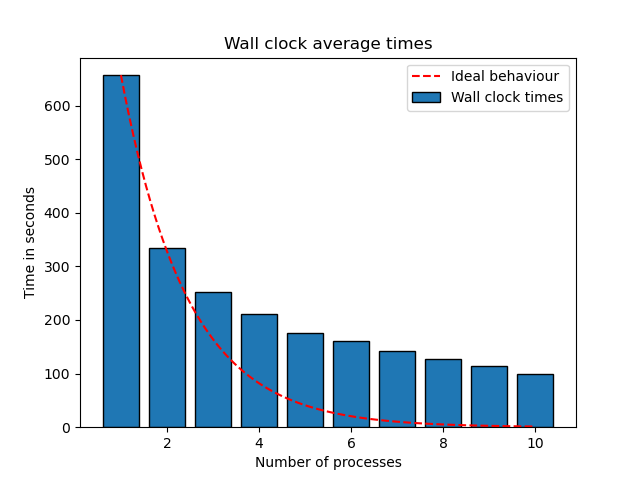
\includegraphics[scale=0.8]{walltimes.png}
\end{figure}


The dotted red line follows curve for the ideal case of parallelization \\$t(p)\sim C\cdot 2^{-p}$
where time halves as number of processes doubles. We can see that this does not happen here for
several reasons. There are some processes which only the root handles, such as the collection of
the best chromosomes. The communication between processes takes time as well. Also, there are more
mutations with more processes. There is however a significant increase in performance, altough the
decrease in time seems to follow more of a linear curve after around 5 processes. The scaling could
also be significantly improved by increasing the migration interval parameter, since the time spent
communicating is directly dependent with it.

There is a balance to be found by testing good values for parameters of the program. Population
size should be large enough so enough results can be explored, but not too big since larger
poipulations size means longer times in computation. Migration interval should be small enough that
genes can spread between processes while keeping the frequency as small as possible to not waste
time in communicating between processes. By doing more tests, the scaling behaviour due to number
of processes as well as the overall cputime could be improved significantly from the current
performance.


\section{Conclusions}

The traveling salesman problem is an important optimization problem, with multiple applications.
By finding solutions to the problem, for example truck routes and computer wiring, can be improved
\cite{Bryant}.

Genetic algorithms can be used to solve a variety of optimization problems, including the traveling
salesman problem. By properly setting up the algorithm, we can efficiently find solutions to
traveling salesman and utilize different tools such as parallelization.

We found that parallelizing the genetic algorithm, we can significantly improve performance and
that tweaking parameters of the program can have a large effect on computation efficiency.

At the end of report is a solution found by run on Ukko:
\begin{lstlisting}
  mpirun -np 12 GA_TSP_parallel 1000 15000 1 30
\end{lstlisting}

\begin{figure}[h]
  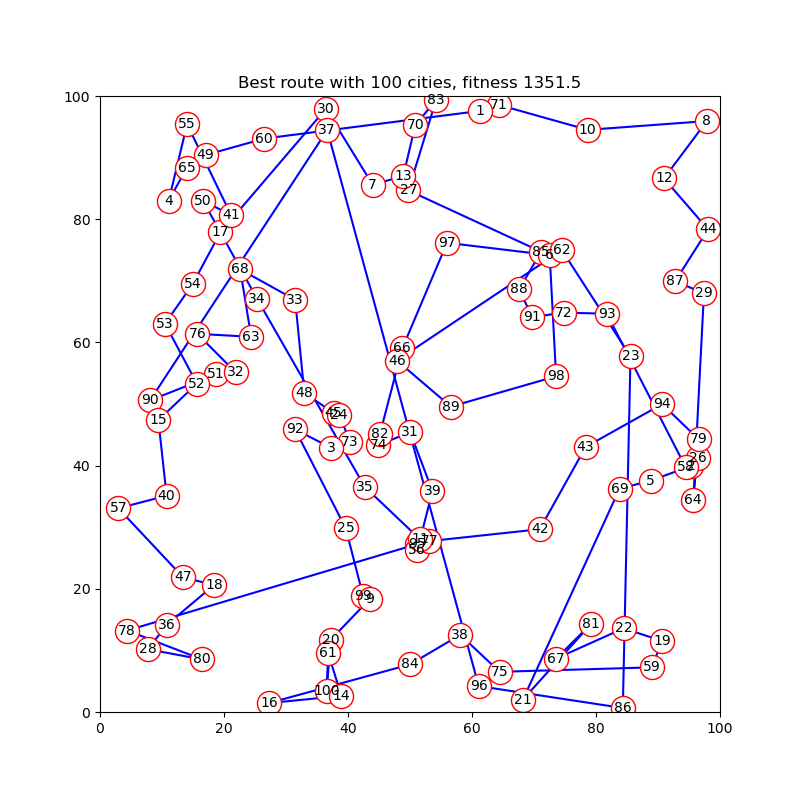
\includegraphics[scale=0.7]{best_chromosome100plot.png}
\end{figure}





\bibliographystyle{alpha}
\bibliography{references}

\end{document}